\section{CodeGlassインターフェース}

\begin{figure*}[t]
\centering
\begin{minipage}{0.49\textwidth}
    \subfloat[関連するプルリクエストの一覧画面.]
    {
        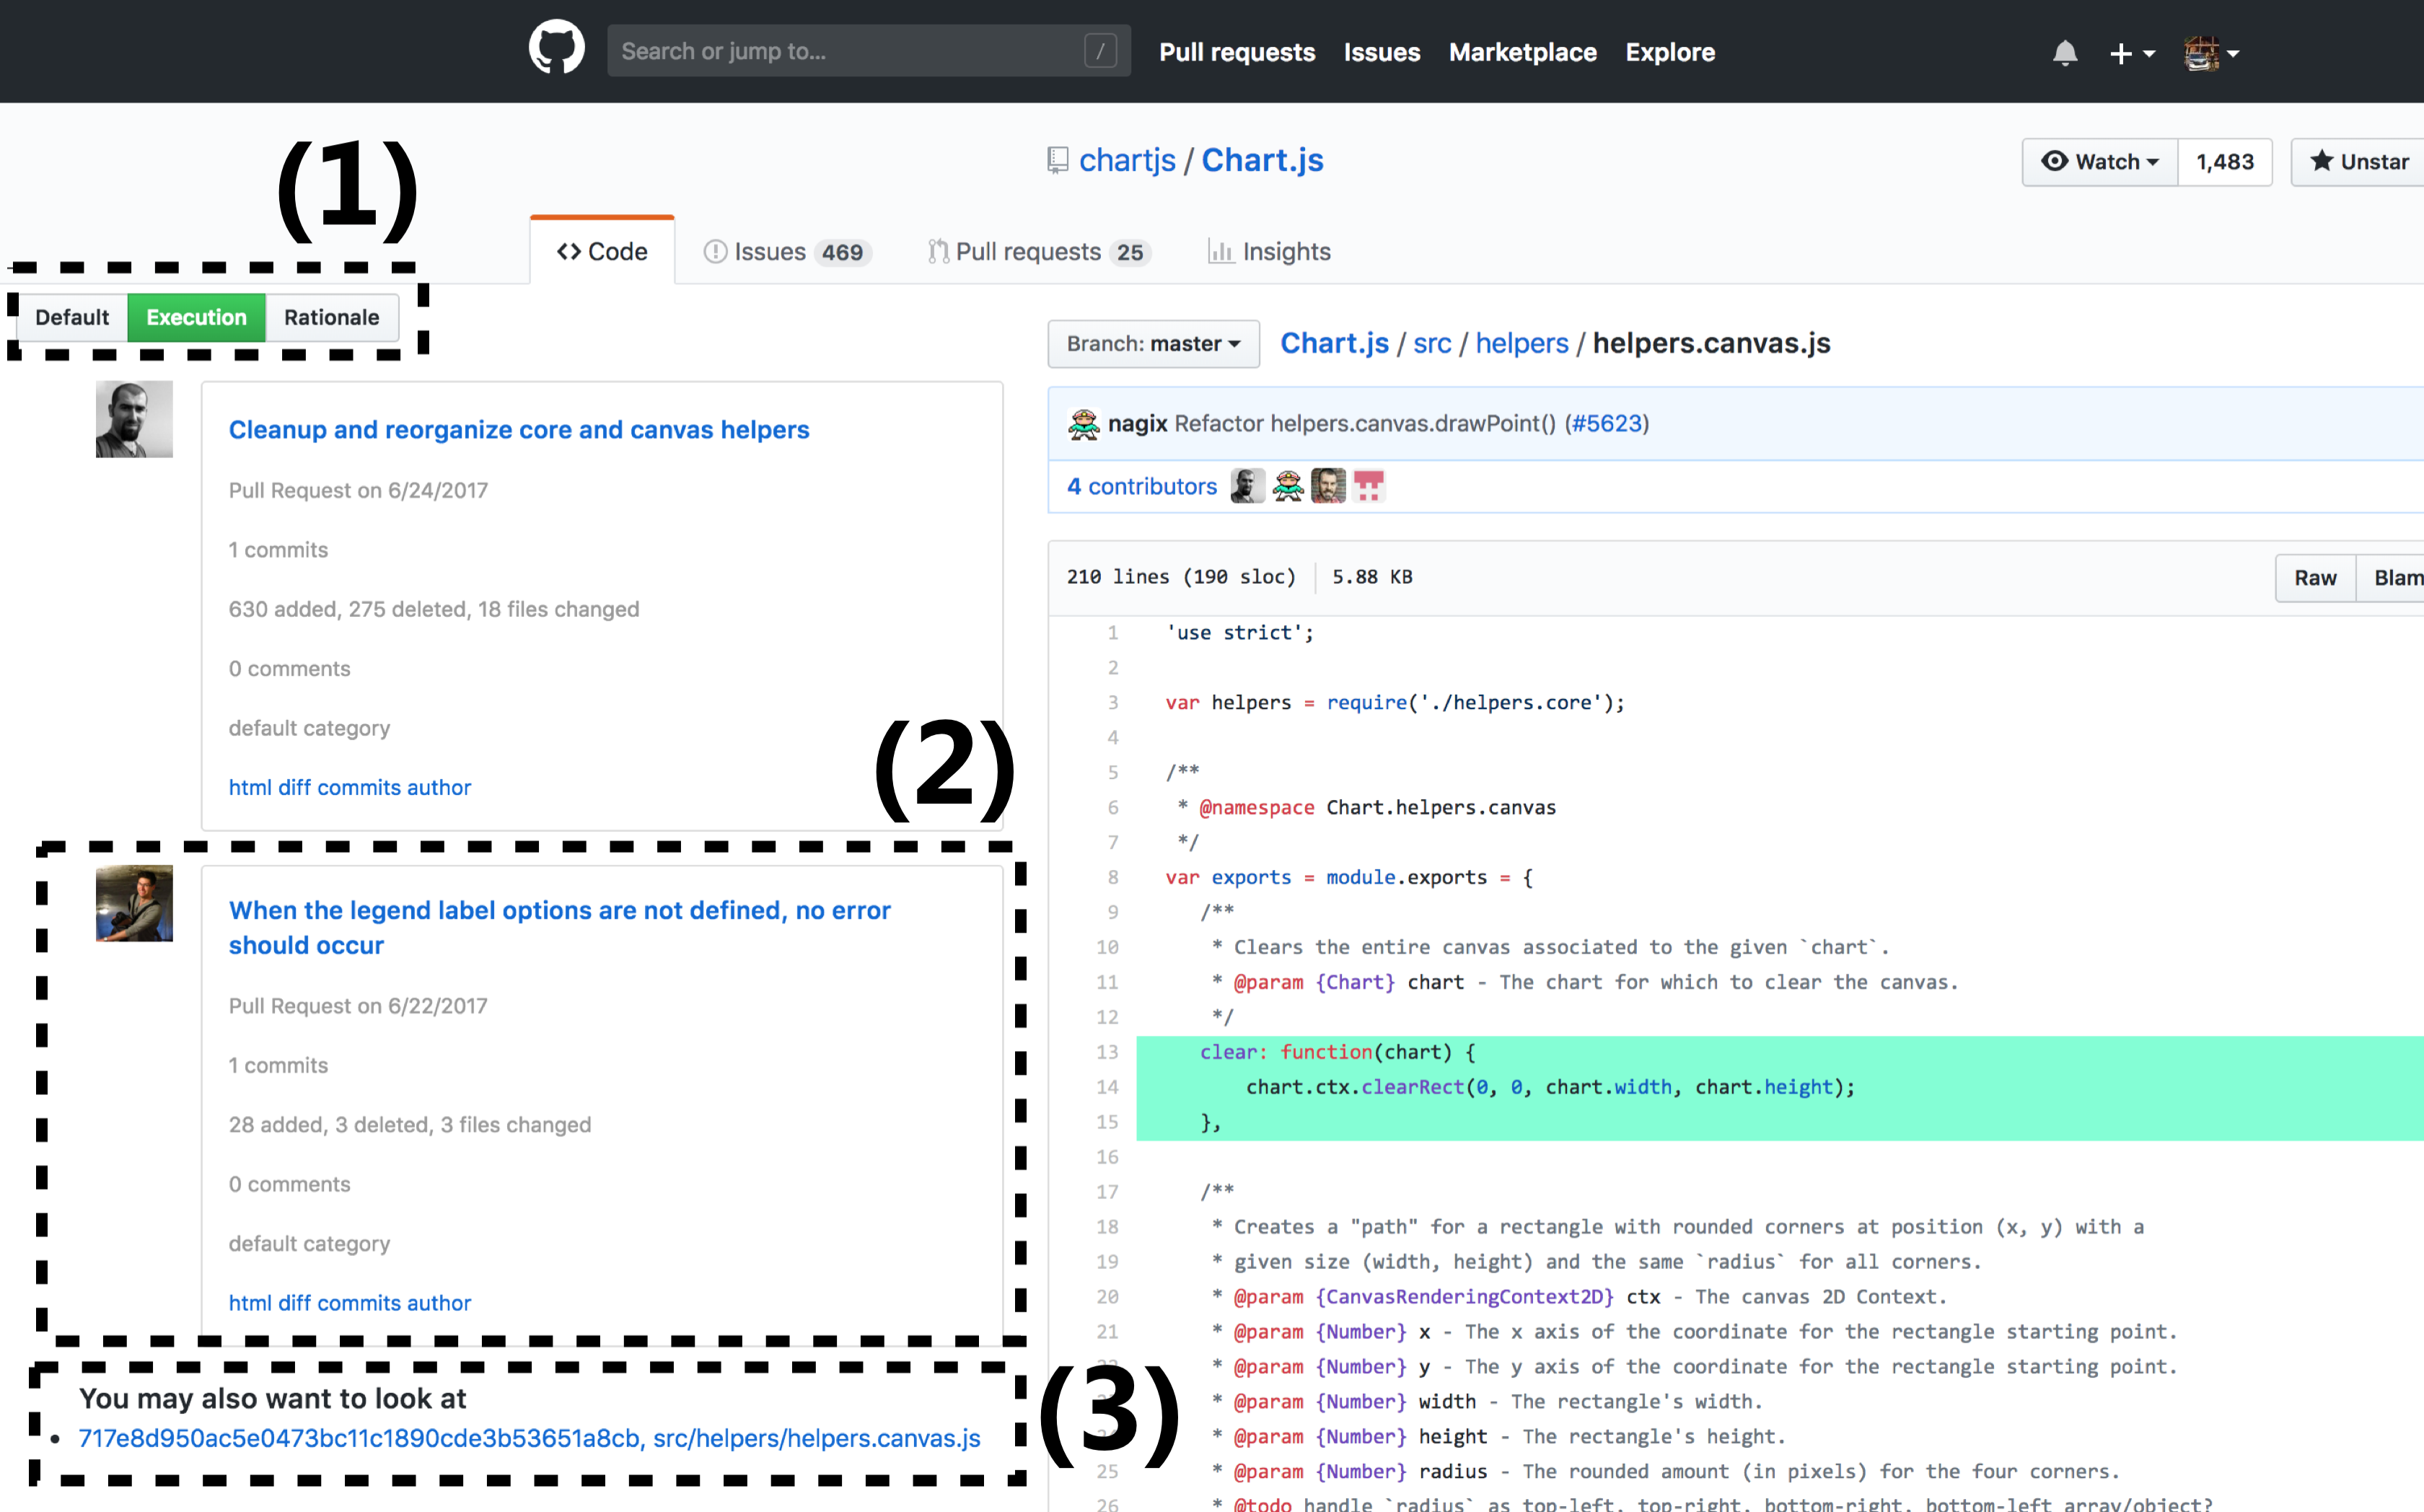
\includegraphics[width=0.95\hsize]{interface/interface1.png}
        \label{fig:interface1}
    }    
\end{minipage}
% \par\hspace{.005\linewidth} 
\begin{minipage}{0.49\textwidth}
    
    \subfloat[プルリクエストの詳細画面.]
    {
        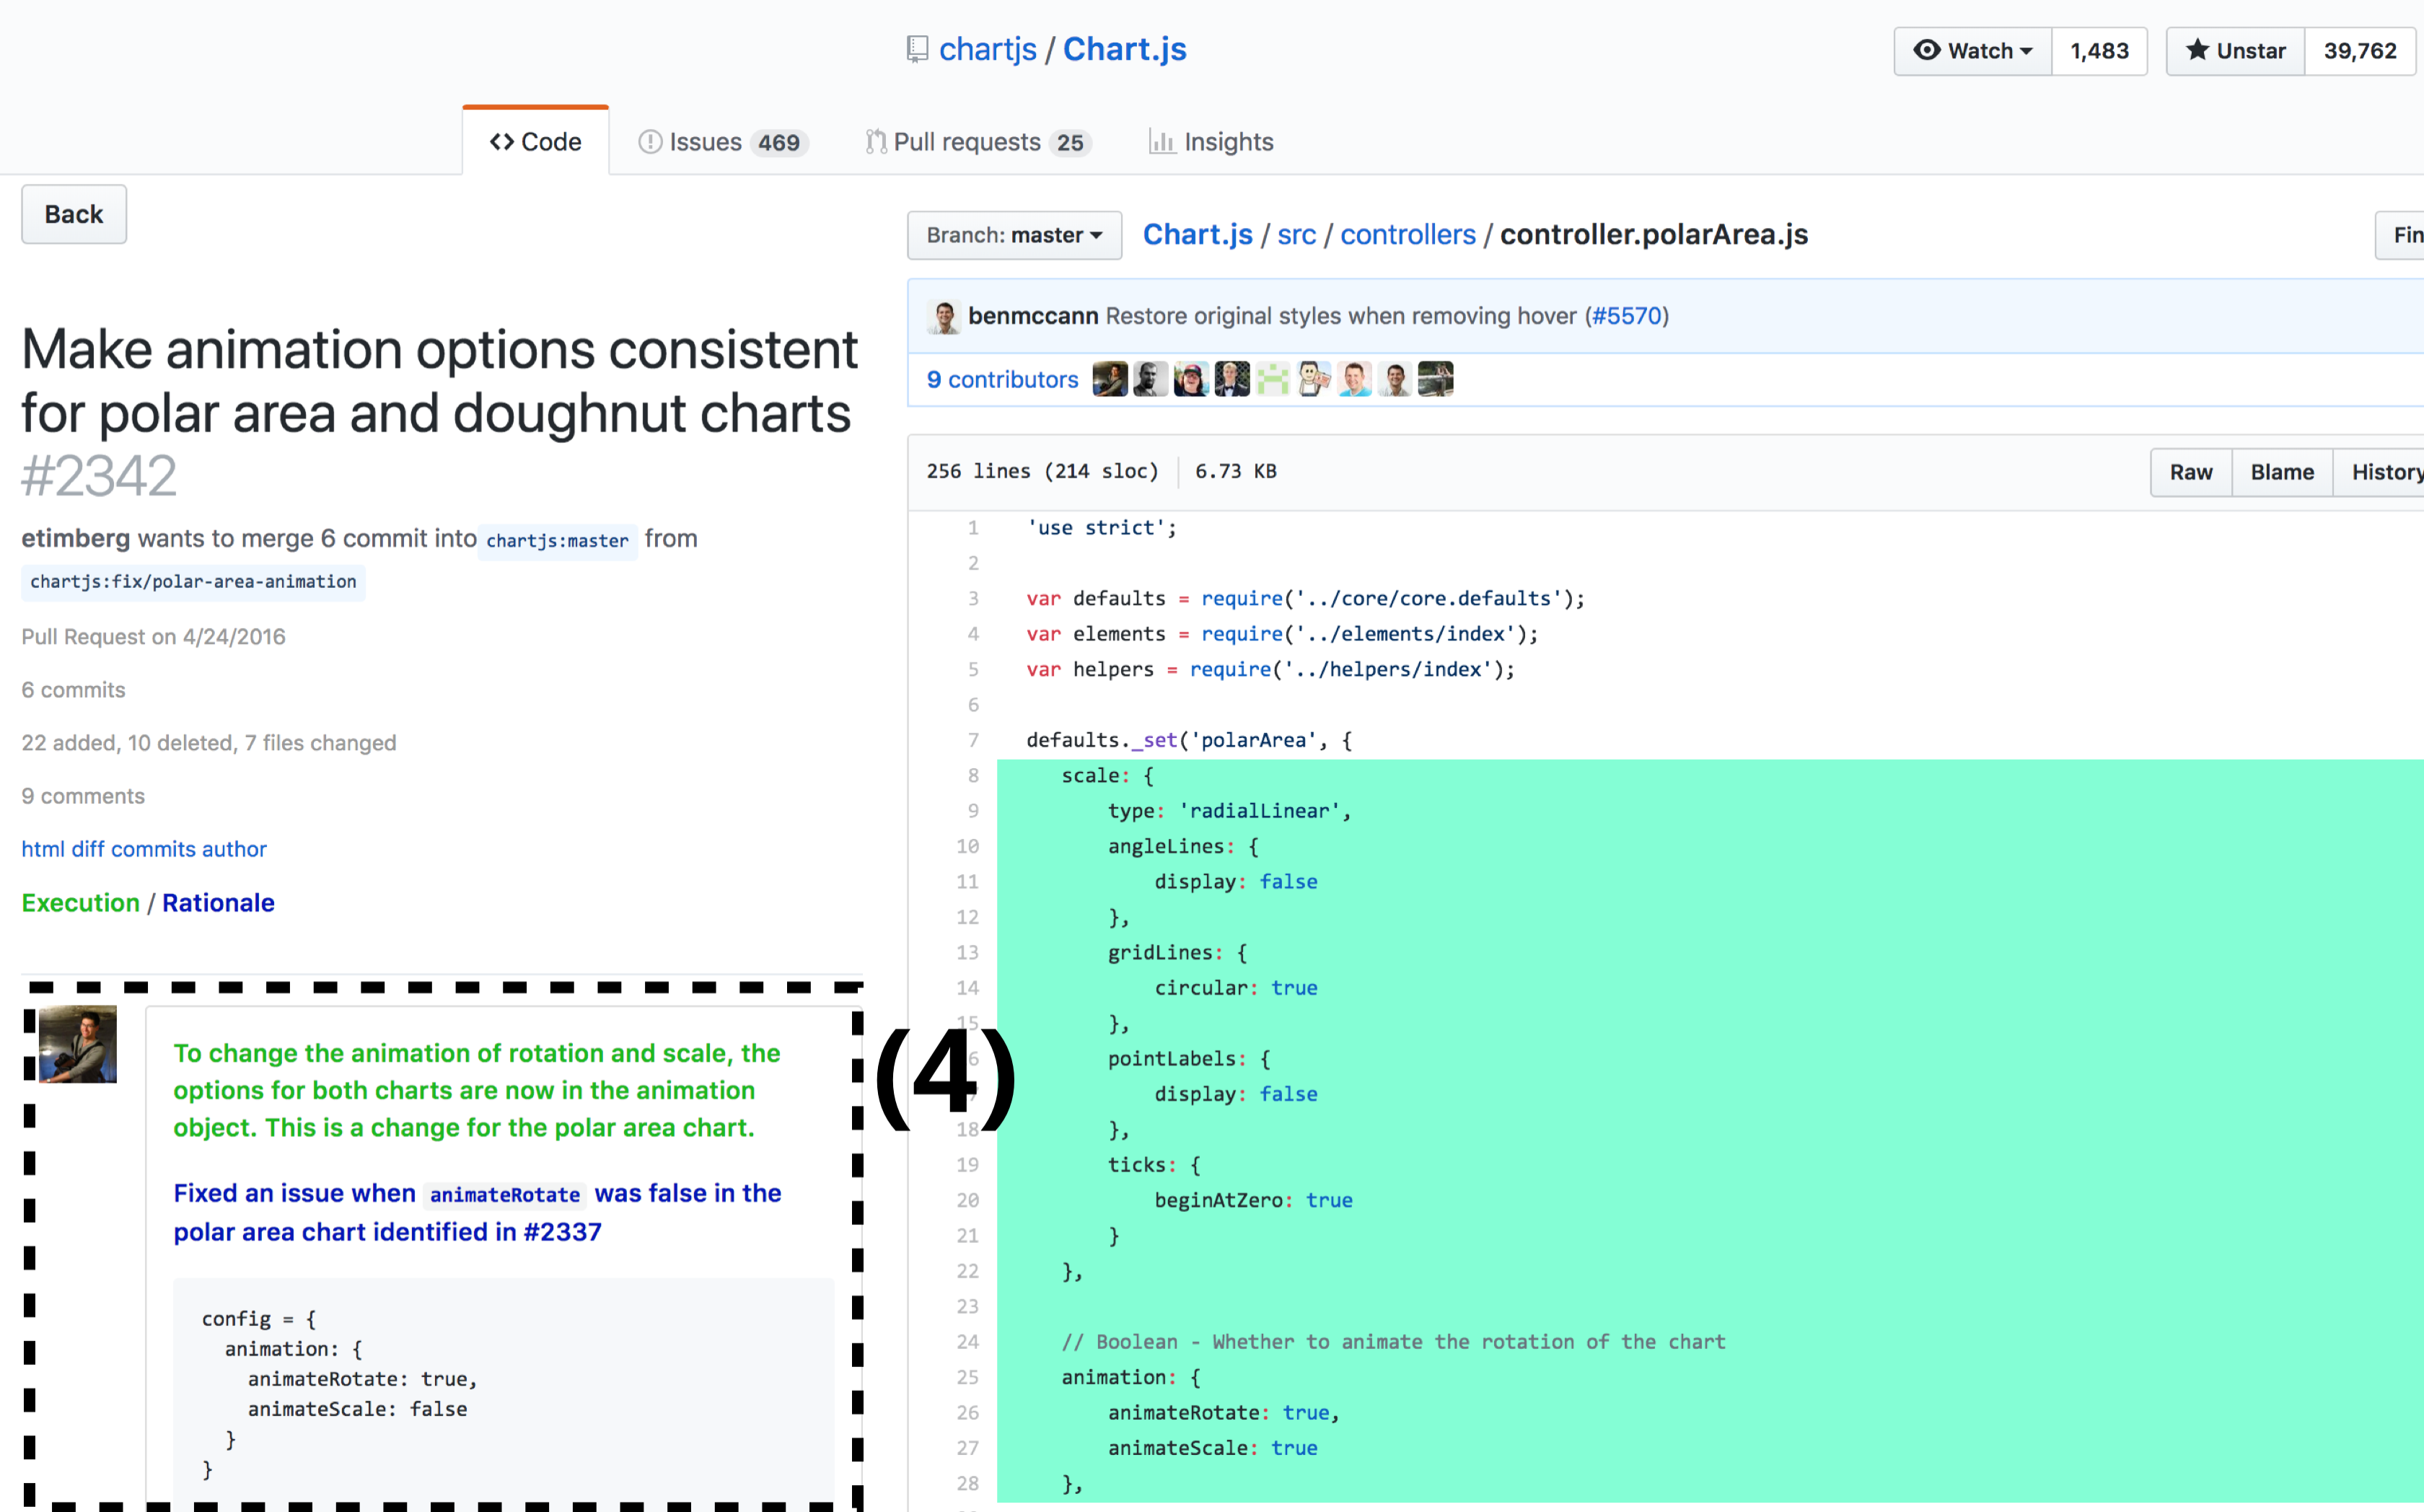
\includegraphics[width=0.95\hsize]{interface/interface2.png}
        \label{fig:interface2}
    }
    
\end{minipage}
	\caption{CodeGlassのインターフェースは,ユーザが選択したコード断片(緑にハイライトされたコード)に関連する過去のプルリクエストの一覧を表示する.抽出されたプルリクエストの表示順は,時系列順,実装内容(Execution)に関する情報が多い順,開発背景(Rationale)に関する情報が多い順に並べることできる~(1).各プルリクエストにはタイトル,コミット数,コードの追加および削除行数,コメント数,そして関連する各ウェブページへのリンクが表示される~(2).さらに,選択されたコード断片と一致する可能性があるコード断片が過去のバージョンの1つで複数ある場合,そのバージョンにおけるソースコードへのリンクが表示される~(3).プルリクエストのタイトルをクリックすると,その詳細情報を確認できる.詳細画面では,プルリクエストの情報に加えて,レビューコメントも表示される.さらに,Executionに分類される文章は緑色で,Rationaleに分類される文章は青色で表示される~(4).}
    \label{fig:WebInterface}
\end{figure*}


CodeGlassはGitHubのプルリクエストを用いてコード断片の理解を支援するインタラクティブなツールである.
本研究におけるコード断片は,ソースコード中の一部の連続したコードである,と定義する.
即ち,コード断片は一行のコードにも,関数やクラス,あるいはファイル全体のコードにもなり得る.
CodeGlassはユーザが選択したコード断片に関連する過去のプルリクエストを抽出し,インターフェースを通じてユーザに提供する.


% We develop an interactive piece-level code examination tool, called CodeGlass.
% The definition of a code piece in this work is consecutive lines in code.
% It can be a single line, function, class or an entire file of code.
% CodeGlass extracts the revision history on the code piece selected by the user.
% Its interface then provides an overview of past pull requests associated with the selected code piece which contain descriptions, commits, and review comments.


図~\ref{fig:WebInterface}にCodeGlassのインターフェースを示す.
ユーザはマウスドラッグでコード断片を指定する(緑でハイライト)事で,関連する過去のプルリクエストやコミットを確認できる(図~\ref{fig:interface1}).
図~\ref{fig:interface1}~(1)に示すボタンから,関連する過去のプルリクエストの表示順を時系列順,実装内容(Execution)に関する情報が多い順,開発背景(Rationale)に関する情報が多い順に並び替えることができる.
これにより,どのように開発が進められてきたか(History)という情報に加えて,実装内容や開発背景を含むと考えられるプルリクエストを強調して提示することも可能となっている.

それぞれのプルリクエストには,タイトルやプルリクエストのID,含まれるコミット数,コードの変更行数,そしてコメント数が表示されている.
また,GitHub上でのプルリクエストや,コード差分,レビューコメント,そしてプルリクエスト作成者へのウェブページへのリンクも示されている.
加えて,図~\ref{fig:interface1}~(3)に示すように,選択されたコード断片と一致する可能性があるコード断片が過去のバージョンの1つで複数ある場合,そのコミットへのリンクも表示する.
ユーザがプルリクエストのタイトルをクリックすると,CodeGlassはその詳細を表示する(図~\ref{fig:interface2}).
詳細画面では,プルリクエストの基本的な情報に加えてレビューコメントも表示される.
また,図~\ref{fig:interface2}~(4)に示すように,プルリクエストの説明文中で実装内容や開発背景に関する情報であると推定された箇所は,色付きの文字で強調される.

% GitHub displays a source code in a file in the red frame in Figure~\ref{fig:WebInterface}.
% CodeGlass provides ``Fetch'' button~(i.e., blue frame in Fig.~\ref{fig:WebInterface}) and a feature that the user can select codes by pointer~(i.e., green frame in Fig.~\ref{fig:WebInterface}).
% Figure~\ref{fig:WebInterface} shows the CodeGlass interface.
% The user specifies a code piece to read descriptions and review comments of past pull requests by a mouse drag~(highlighted in light green in Figure~\ref{fig:WebInterface}).
% CodeGlass displays a series of relevant pull requests in the chronological order as shown in Figure~\ref{fig:WebInterface}a.
% Each pull request is summarized in a separate box ((1) in Figure~\ref{fig:WebInterface}a).
% Each summary includes the title of a pull request, its ID, and the numbers of commits, lines and files changed, and comments.
% It also contains links to the original pull request page, the diff summary, review comments, and the author's page to allow the user to further investigate details.
% In addition, CodeGlass suggests other potentially-relevant commits if there exists any ((2) in Figure~\ref{fig:WebInterface}a).
% When clicking one of them, the user can view the version associated with the selected commit and further investigate how code has been developed.
% When the user clicks the title of a pull request summary, CodeGlass presents its review comments ((3) in Figure~\ref{fig:WebInterface}b).

CodeGlassにおいてユーザは,クラスや関数といった単位に縛られる事なく自由にコード断片を選択し,関連する過去のプルリクエストを調べる事ができる.
特にユーザが大きなクラスや関数のコードを調査する際には,自由にコードを分割して調べる事ができるため有用であると考える.
CodeGlassはプログラミング言語に依存する事なく動作するため,GitHub上の全てのオープンなリポジトリに対して,CodeGlassのサーバにリポジトリをクローンする事で利用可能となっている.
アクセス制限などを設定する事で,技術的にはプライベートリポジトリにも対応する事ができる.


% CodeGlass allows developers to examine past pull requests and commits on any line of code, not limited to meaningful chunks (e.g., classes or functions).
% This capability is useful when developers need to investigate large classes and functions because they can have freedom to break down into smaller portions for their examination.

% 現在のCodeGlassのプロトタイプはサーバとインターフェースの二つに分けて実装されている.
% インターフェースはGoogle Chromeの拡張機能として開発されている.
% サーバはインターフェースからリポジトリ名やファイル名,選択されたコード断片の位置を受け取り,それらに関連する過去のプルリクエストをインターフェースに返す仕組みとなっている.

% CodeGlassはプログラミング言語に依存する事なく動作するため,GitHub上の全てのオープンなリポジトリに対して,CodeGlassのサーバにリポジトリをクローンする事で動作する事が可能となっている.
% アクセス制限などを設定する事で,技術的にはプライベートリポジトリにも対応する事が出来る.


% The current CodeGlass system takes a server-client implementation.
% The CodeGlass interface is implemented as a Google Chrome extension.
% The server accepts information necessary for search (e.g., the repository name, file name, and line numbers) upon user's selection of a code piece, and returns relevant pull request data.

%Our current prototype would function for any public repository on GitHub because the backend algorithm is language-agnostic as we explain later.
%With proper permission settings, CodeGlass would be available even for private repositories.
% There are 57 million active repositories as of April 2017\footnote{\url{https://github.com/blog/2345-celebrating-nine-years-of-\\github-with-an-anniversary-sale}}.








